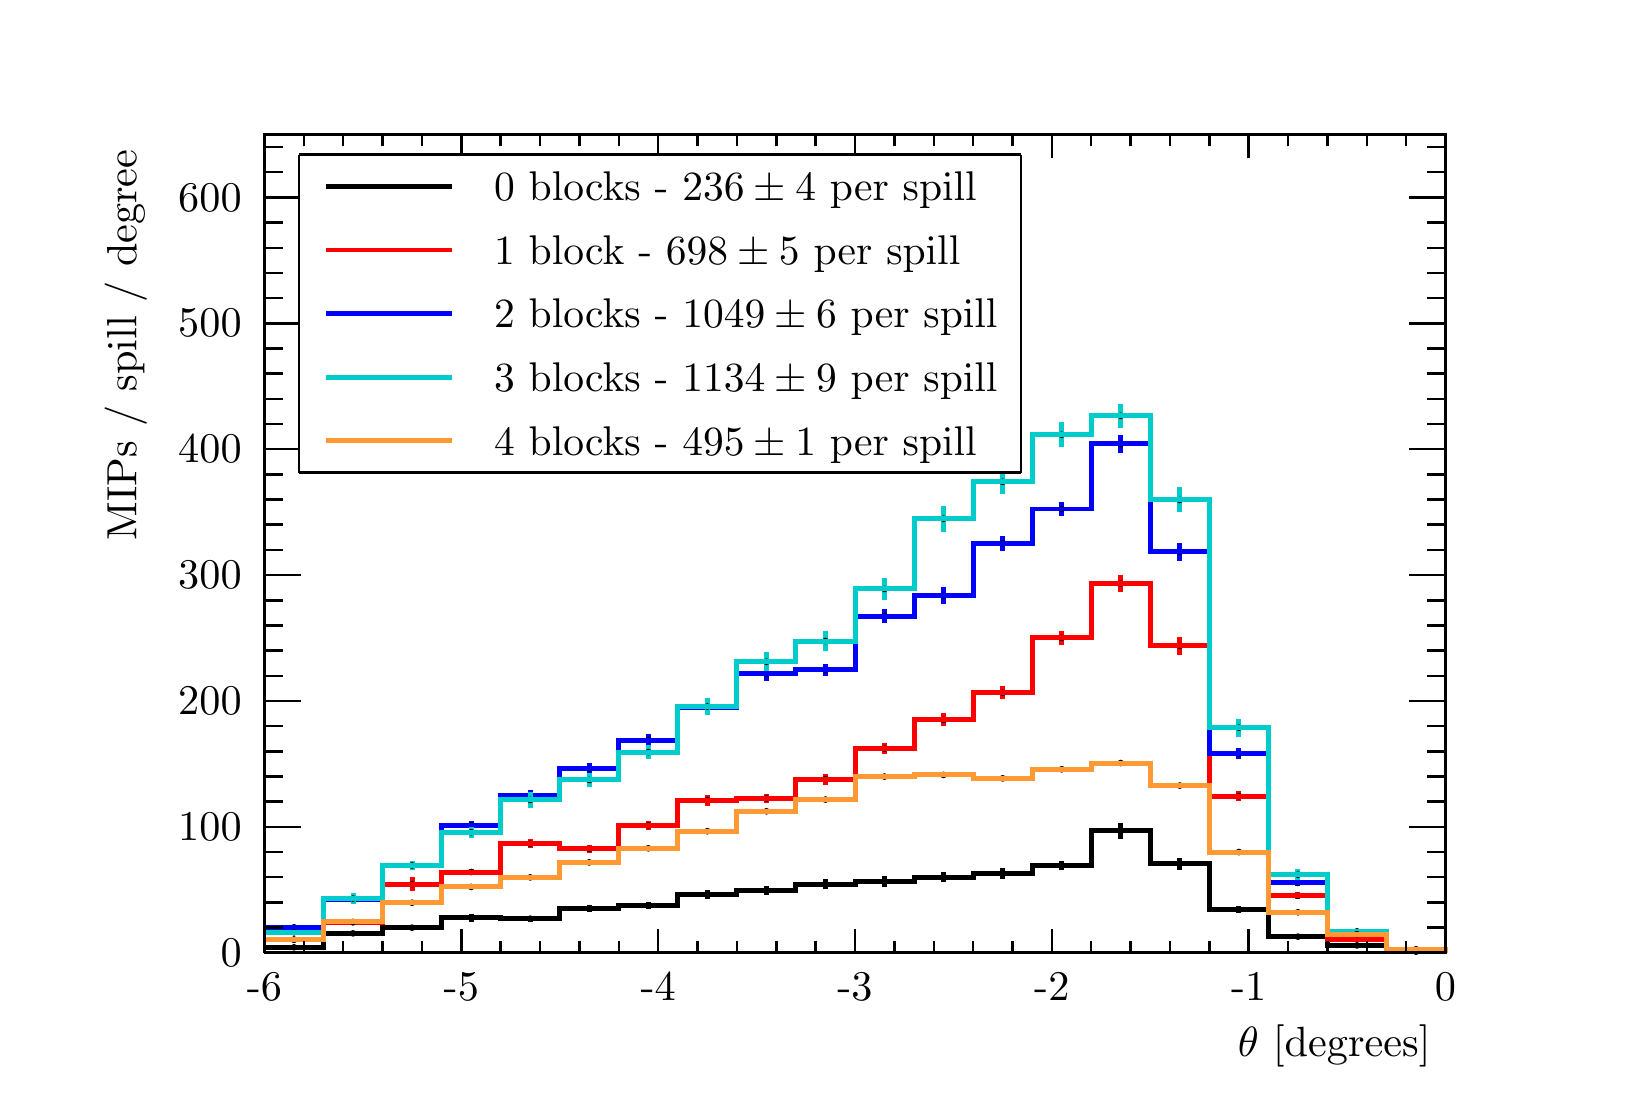
\begin{tikzpicture}
\pgfdeclareplotmark{cross} {
\pgfpathmoveto{\pgfpoint{-0.3\pgfplotmarksize}{\pgfplotmarksize}}
\pgfpathlineto{\pgfpoint{+0.3\pgfplotmarksize}{\pgfplotmarksize}}
\pgfpathlineto{\pgfpoint{+0.3\pgfplotmarksize}{0.3\pgfplotmarksize}}
\pgfpathlineto{\pgfpoint{+1\pgfplotmarksize}{0.3\pgfplotmarksize}}
\pgfpathlineto{\pgfpoint{+1\pgfplotmarksize}{-0.3\pgfplotmarksize}}
\pgfpathlineto{\pgfpoint{+0.3\pgfplotmarksize}{-0.3\pgfplotmarksize}}
\pgfpathlineto{\pgfpoint{+0.3\pgfplotmarksize}{-1.\pgfplotmarksize}}
\pgfpathlineto{\pgfpoint{-0.3\pgfplotmarksize}{-1.\pgfplotmarksize}}
\pgfpathlineto{\pgfpoint{-0.3\pgfplotmarksize}{-0.3\pgfplotmarksize}}
\pgfpathlineto{\pgfpoint{-1.\pgfplotmarksize}{-0.3\pgfplotmarksize}}
\pgfpathlineto{\pgfpoint{-1.\pgfplotmarksize}{0.3\pgfplotmarksize}}
\pgfpathlineto{\pgfpoint{-0.3\pgfplotmarksize}{0.3\pgfplotmarksize}}
\pgfpathclose
\pgfusepathqstroke
}
\pgfdeclareplotmark{cross*} {
\pgfpathmoveto{\pgfpoint{-0.3\pgfplotmarksize}{\pgfplotmarksize}}
\pgfpathlineto{\pgfpoint{+0.3\pgfplotmarksize}{\pgfplotmarksize}}
\pgfpathlineto{\pgfpoint{+0.3\pgfplotmarksize}{0.3\pgfplotmarksize}}
\pgfpathlineto{\pgfpoint{+1\pgfplotmarksize}{0.3\pgfplotmarksize}}
\pgfpathlineto{\pgfpoint{+1\pgfplotmarksize}{-0.3\pgfplotmarksize}}
\pgfpathlineto{\pgfpoint{+0.3\pgfplotmarksize}{-0.3\pgfplotmarksize}}
\pgfpathlineto{\pgfpoint{+0.3\pgfplotmarksize}{-1.\pgfplotmarksize}}
\pgfpathlineto{\pgfpoint{-0.3\pgfplotmarksize}{-1.\pgfplotmarksize}}
\pgfpathlineto{\pgfpoint{-0.3\pgfplotmarksize}{-0.3\pgfplotmarksize}}
\pgfpathlineto{\pgfpoint{-1.\pgfplotmarksize}{-0.3\pgfplotmarksize}}
\pgfpathlineto{\pgfpoint{-1.\pgfplotmarksize}{0.3\pgfplotmarksize}}
\pgfpathlineto{\pgfpoint{-0.3\pgfplotmarksize}{0.3\pgfplotmarksize}}
\pgfpathclose
\pgfusepathqfillstroke
}
\pgfdeclareplotmark{newstar} {
\pgfpathmoveto{\pgfqpoint{0pt}{\pgfplotmarksize}}
\pgfpathlineto{\pgfqpointpolar{44}{0.5\pgfplotmarksize}}
\pgfpathlineto{\pgfqpointpolar{18}{\pgfplotmarksize}}
\pgfpathlineto{\pgfqpointpolar{-20}{0.5\pgfplotmarksize}}
\pgfpathlineto{\pgfqpointpolar{-54}{\pgfplotmarksize}}
\pgfpathlineto{\pgfqpointpolar{-90}{0.5\pgfplotmarksize}}
\pgfpathlineto{\pgfqpointpolar{234}{\pgfplotmarksize}}
\pgfpathlineto{\pgfqpointpolar{198}{0.5\pgfplotmarksize}}
\pgfpathlineto{\pgfqpointpolar{162}{\pgfplotmarksize}}
\pgfpathlineto{\pgfqpointpolar{134}{0.5\pgfplotmarksize}}
\pgfpathclose
\pgfusepathqstroke
}
\pgfdeclareplotmark{newstar*} {
\pgfpathmoveto{\pgfqpoint{0pt}{\pgfplotmarksize}}
\pgfpathlineto{\pgfqpointpolar{44}{0.5\pgfplotmarksize}}
\pgfpathlineto{\pgfqpointpolar{18}{\pgfplotmarksize}}
\pgfpathlineto{\pgfqpointpolar{-20}{0.5\pgfplotmarksize}}
\pgfpathlineto{\pgfqpointpolar{-54}{\pgfplotmarksize}}
\pgfpathlineto{\pgfqpointpolar{-90}{0.5\pgfplotmarksize}}
\pgfpathlineto{\pgfqpointpolar{234}{\pgfplotmarksize}}
\pgfpathlineto{\pgfqpointpolar{198}{0.5\pgfplotmarksize}}
\pgfpathlineto{\pgfqpointpolar{162}{\pgfplotmarksize}}
\pgfpathlineto{\pgfqpointpolar{134}{0.5\pgfplotmarksize}}
\pgfpathclose
\pgfusepathqfillstroke
}
\definecolor{c}{rgb}{1,1,1};
\draw [color=c, fill=c] (0,0) rectangle (20,13.4957);
\draw [color=c, fill=c] (3,1.75444) rectangle (18,12.1461);
\definecolor{c}{rgb}{0,0,0};
\draw [c,line width=0.9] (3,1.75444) -- (3,12.1461) -- (18,12.1461) -- (18,1.75444) -- (3,1.75444);
\definecolor{c}{rgb}{1,1,1};
\draw [color=c, fill=c] (3,1.75444) rectangle (18,12.1461);
\definecolor{c}{rgb}{0,0,0};
\draw [c,line width=0.9] (3,1.75444) -- (3,12.1461) -- (18,12.1461) -- (18,1.75444) -- (3,1.75444);
\draw [c,line width=0.9] (3,1.75444) -- (3.75,1.75444) -- (3.75,1.75444) -- (4.5,1.75444) -- (4.5,1.75444) -- (5.25,1.75444) -- (5.25,1.75444) -- (6,1.75444) -- (6,1.75444) -- (6.75,1.75444) -- (6.75,1.75444) -- (7.5,1.75444) -- (7.5,1.75444) --
 (8.25,1.75444) -- (8.25,1.75444) -- (9,1.75444) -- (9,1.75444) -- (9.75,1.75444) -- (9.75,1.75444) -- (10.5,1.75444) -- (10.5,1.75444) -- (11.25,1.75444) -- (11.25,1.75444) -- (12,1.75444) -- (12,1.75444) -- (12.75,1.75444) -- (12.75,1.75444) --
 (13.5,1.75444) -- (13.5,1.75444) -- (14.25,1.75444) -- (14.25,1.75444) -- (15,1.75444) -- (15,1.75444) -- (15.75,1.75444) -- (15.75,1.75444) -- (16.5,1.75444) -- (16.5,1.75444) -- (17.25,1.75444) -- (17.25,1.75444) -- (18,1.75444) -- (18,1.75444);
\draw [c,line width=0.9] (3,1.75444) -- (18,1.75444);
\draw [c,line width=0.9] (3,2.05809) -- (3,1.75444);
\draw [c,line width=0.9] (3.5,1.90627) -- (3.5,1.75444);
\draw [c,line width=0.9] (4,1.90627) -- (4,1.75444);
\draw [c,line width=0.9] (4.5,1.90627) -- (4.5,1.75444);
\draw [c,line width=0.9] (5,1.90627) -- (5,1.75444);
\draw [c,line width=0.9] (5.5,2.05809) -- (5.5,1.75444);
\draw [c,line width=0.9] (6,1.90627) -- (6,1.75444);
\draw [c,line width=0.9] (6.5,1.90627) -- (6.5,1.75444);
\draw [c,line width=0.9] (7,1.90627) -- (7,1.75444);
\draw [c,line width=0.9] (7.5,1.90627) -- (7.5,1.75444);
\draw [c,line width=0.9] (8,2.05809) -- (8,1.75444);
\draw [c,line width=0.9] (8.5,1.90627) -- (8.5,1.75444);
\draw [c,line width=0.9] (9,1.90627) -- (9,1.75444);
\draw [c,line width=0.9] (9.5,1.90627) -- (9.5,1.75444);
\draw [c,line width=0.9] (10,1.90627) -- (10,1.75444);
\draw [c,line width=0.9] (10.5,2.05809) -- (10.5,1.75444);
\draw [c,line width=0.9] (11,1.90627) -- (11,1.75444);
\draw [c,line width=0.9] (11.5,1.90627) -- (11.5,1.75444);
\draw [c,line width=0.9] (12,1.90627) -- (12,1.75444);
\draw [c,line width=0.9] (12.5,1.90627) -- (12.5,1.75444);
\draw [c,line width=0.9] (13,2.05809) -- (13,1.75444);
\draw [c,line width=0.9] (13.5,1.90627) -- (13.5,1.75444);
\draw [c,line width=0.9] (14,1.90627) -- (14,1.75444);
\draw [c,line width=0.9] (14.5,1.90627) -- (14.5,1.75444);
\draw [c,line width=0.9] (15,1.90627) -- (15,1.75444);
\draw [c,line width=0.9] (15.5,2.05809) -- (15.5,1.75444);
\draw [c,line width=0.9] (16,1.90627) -- (16,1.75444);
\draw [c,line width=0.9] (16.5,1.90627) -- (16.5,1.75444);
\draw [c,line width=0.9] (17,1.90627) -- (17,1.75444);
\draw [c,line width=0.9] (17.5,1.90627) -- (17.5,1.75444);
\draw [c,line width=0.9] (18,2.05809) -- (18,1.75444);
\draw [anchor=base] (3,1.14713) node[scale=1.52731, color=c, rotate=0]{-6};
\draw [anchor=base] (5.5,1.14713) node[scale=1.52731, color=c, rotate=0]{-5};
\draw [anchor=base] (8,1.14713) node[scale=1.52731, color=c, rotate=0]{-4};
\draw [anchor=base] (10.5,1.14713) node[scale=1.52731, color=c, rotate=0]{-3};
\draw [anchor=base] (13,1.14713) node[scale=1.52731, color=c, rotate=0]{-2};
\draw [anchor=base] (15.5,1.14713) node[scale=1.52731, color=c, rotate=0]{-1};
\draw [anchor=base] (18,1.14713) node[scale=1.52731, color=c, rotate=0]{0};
\draw [anchor= east] (18,0.566819) node[scale=1.52731, color=c, rotate=0]{$\theta$ [degrees]};
\draw [c,line width=0.9] (3,12.1461) -- (18,12.1461);
\draw [c,line width=0.9] (3,11.8425) -- (3,12.1461);
\draw [c,line width=0.9] (3.5,11.9943) -- (3.5,12.1461);
\draw [c,line width=0.9] (4,11.9943) -- (4,12.1461);
\draw [c,line width=0.9] (4.5,11.9943) -- (4.5,12.1461);
\draw [c,line width=0.9] (5,11.9943) -- (5,12.1461);
\draw [c,line width=0.9] (5.5,11.8425) -- (5.5,12.1461);
\draw [c,line width=0.9] (6,11.9943) -- (6,12.1461);
\draw [c,line width=0.9] (6.5,11.9943) -- (6.5,12.1461);
\draw [c,line width=0.9] (7,11.9943) -- (7,12.1461);
\draw [c,line width=0.9] (7.5,11.9943) -- (7.5,12.1461);
\draw [c,line width=0.9] (8,11.8425) -- (8,12.1461);
\draw [c,line width=0.9] (8.5,11.9943) -- (8.5,12.1461);
\draw [c,line width=0.9] (9,11.9943) -- (9,12.1461);
\draw [c,line width=0.9] (9.5,11.9943) -- (9.5,12.1461);
\draw [c,line width=0.9] (10,11.9943) -- (10,12.1461);
\draw [c,line width=0.9] (10.5,11.8425) -- (10.5,12.1461);
\draw [c,line width=0.9] (11,11.9943) -- (11,12.1461);
\draw [c,line width=0.9] (11.5,11.9943) -- (11.5,12.1461);
\draw [c,line width=0.9] (12,11.9943) -- (12,12.1461);
\draw [c,line width=0.9] (12.5,11.9943) -- (12.5,12.1461);
\draw [c,line width=0.9] (13,11.8425) -- (13,12.1461);
\draw [c,line width=0.9] (13.5,11.9943) -- (13.5,12.1461);
\draw [c,line width=0.9] (14,11.9943) -- (14,12.1461);
\draw [c,line width=0.9] (14.5,11.9943) -- (14.5,12.1461);
\draw [c,line width=0.9] (15,11.9943) -- (15,12.1461);
\draw [c,line width=0.9] (15.5,11.8425) -- (15.5,12.1461);
\draw [c,line width=0.9] (16,11.9943) -- (16,12.1461);
\draw [c,line width=0.9] (16.5,11.9943) -- (16.5,12.1461);
\draw [c,line width=0.9] (17,11.9943) -- (17,12.1461);
\draw [c,line width=0.9] (17.5,11.9943) -- (17.5,12.1461);
\draw [c,line width=0.9] (18,11.8425) -- (18,12.1461);
\draw [c,line width=0.9] (3,1.75444) -- (3,12.1461);
\draw [c,line width=0.9] (3.462,1.75444) -- (3,1.75444);
\draw [c,line width=0.9] (3.231,2.07419) -- (3,2.07419);
\draw [c,line width=0.9] (3.231,2.39393) -- (3,2.39393);
\draw [c,line width=0.9] (3.231,2.71367) -- (3,2.71367);
\draw [c,line width=0.9] (3.231,3.03342) -- (3,3.03342);
\draw [c,line width=0.9] (3.462,3.35316) -- (3,3.35316);
\draw [c,line width=0.9] (3.231,3.67291) -- (3,3.67291);
\draw [c,line width=0.9] (3.231,3.99265) -- (3,3.99265);
\draw [c,line width=0.9] (3.231,4.3124) -- (3,4.3124);
\draw [c,line width=0.9] (3.231,4.63214) -- (3,4.63214);
\draw [c,line width=0.9] (3.462,4.95188) -- (3,4.95188);
\draw [c,line width=0.9] (3.231,5.27163) -- (3,5.27163);
\draw [c,line width=0.9] (3.231,5.59137) -- (3,5.59137);
\draw [c,line width=0.9] (3.231,5.91112) -- (3,5.91112);
\draw [c,line width=0.9] (3.231,6.23086) -- (3,6.23086);
\draw [c,line width=0.9] (3.462,6.55061) -- (3,6.55061);
\draw [c,line width=0.9] (3.231,6.87035) -- (3,6.87035);
\draw [c,line width=0.9] (3.231,7.19009) -- (3,7.19009);
\draw [c,line width=0.9] (3.231,7.50984) -- (3,7.50984);
\draw [c,line width=0.9] (3.231,7.82958) -- (3,7.82958);
\draw [c,line width=0.9] (3.462,8.14933) -- (3,8.14933);
\draw [c,line width=0.9] (3.231,8.46907) -- (3,8.46907);
\draw [c,line width=0.9] (3.231,8.78882) -- (3,8.78882);
\draw [c,line width=0.9] (3.231,9.10856) -- (3,9.10856);
\draw [c,line width=0.9] (3.231,9.4283) -- (3,9.4283);
\draw [c,line width=0.9] (3.462,9.74805) -- (3,9.74805);
\draw [c,line width=0.9] (3.231,10.0678) -- (3,10.0678);
\draw [c,line width=0.9] (3.231,10.3875) -- (3,10.3875);
\draw [c,line width=0.9] (3.231,10.7073) -- (3,10.7073);
\draw [c,line width=0.9] (3.231,11.027) -- (3,11.027);
\draw [c,line width=0.9] (3.462,11.3468) -- (3,11.3468);
\draw [c,line width=0.9] (3.462,11.3468) -- (3,11.3468);
\draw [c,line width=0.9] (3.231,11.6665) -- (3,11.6665);
\draw [c,line width=0.9] (3.231,11.9863) -- (3,11.9863);
\draw [anchor= east] (2.9,1.75444) node[scale=1.52731, color=c, rotate=0]{0};
\draw [anchor= east] (2.9,3.35316) node[scale=1.52731, color=c, rotate=0]{100};
\draw [anchor= east] (2.9,4.95188) node[scale=1.52731, color=c, rotate=0]{200};
\draw [anchor= east] (2.9,6.55061) node[scale=1.52731, color=c, rotate=0]{300};
\draw [anchor= east] (2.9,8.14933) node[scale=1.52731, color=c, rotate=0]{400};
\draw [anchor= east] (2.9,9.74805) node[scale=1.52731, color=c, rotate=0]{500};
\draw [anchor= east] (2.9,11.3468) node[scale=1.52731, color=c, rotate=0]{600};
\draw [anchor= east] (1.24,12.1461) node[scale=1.52731, color=c, rotate=90]{ MIPs / spill / degree};
\draw [c,line width=0.9] (18,1.75444) -- (18,12.1461);
\draw [c,line width=0.9] (17.538,1.75444) -- (18,1.75444);
\draw [c,line width=0.9] (17.769,2.07419) -- (18,2.07419);
\draw [c,line width=0.9] (17.769,2.39393) -- (18,2.39393);
\draw [c,line width=0.9] (17.769,2.71367) -- (18,2.71367);
\draw [c,line width=0.9] (17.769,3.03342) -- (18,3.03342);
\draw [c,line width=0.9] (17.538,3.35316) -- (18,3.35316);
\draw [c,line width=0.9] (17.769,3.67291) -- (18,3.67291);
\draw [c,line width=0.9] (17.769,3.99265) -- (18,3.99265);
\draw [c,line width=0.9] (17.769,4.3124) -- (18,4.3124);
\draw [c,line width=0.9] (17.769,4.63214) -- (18,4.63214);
\draw [c,line width=0.9] (17.538,4.95188) -- (18,4.95188);
\draw [c,line width=0.9] (17.769,5.27163) -- (18,5.27163);
\draw [c,line width=0.9] (17.769,5.59137) -- (18,5.59137);
\draw [c,line width=0.9] (17.769,5.91112) -- (18,5.91112);
\draw [c,line width=0.9] (17.769,6.23086) -- (18,6.23086);
\draw [c,line width=0.9] (17.538,6.55061) -- (18,6.55061);
\draw [c,line width=0.9] (17.769,6.87035) -- (18,6.87035);
\draw [c,line width=0.9] (17.769,7.19009) -- (18,7.19009);
\draw [c,line width=0.9] (17.769,7.50984) -- (18,7.50984);
\draw [c,line width=0.9] (17.769,7.82958) -- (18,7.82958);
\draw [c,line width=0.9] (17.538,8.14933) -- (18,8.14933);
\draw [c,line width=0.9] (17.769,8.46907) -- (18,8.46907);
\draw [c,line width=0.9] (17.769,8.78882) -- (18,8.78882);
\draw [c,line width=0.9] (17.769,9.10856) -- (18,9.10856);
\draw [c,line width=0.9] (17.769,9.4283) -- (18,9.4283);
\draw [c,line width=0.9] (17.538,9.74805) -- (18,9.74805);
\draw [c,line width=0.9] (17.769,10.0678) -- (18,10.0678);
\draw [c,line width=0.9] (17.769,10.3875) -- (18,10.3875);
\draw [c,line width=0.9] (17.769,10.7073) -- (18,10.7073);
\draw [c,line width=0.9] (17.769,11.027) -- (18,11.027);
\draw [c,line width=0.9] (17.538,11.3468) -- (18,11.3468);
\draw [c,line width=0.9] (17.538,11.3468) -- (18,11.3468);
\draw [c,line width=0.9] (17.769,11.6665) -- (18,11.6665);
\draw [c,line width=0.9] (17.769,11.9863) -- (18,11.9863);
\draw [c,line width=1.8] (3.375,1.81609) -- (3.375,1.82333);
\draw [c,line width=1.8] (3.375,1.82333) -- (3.375,1.83057);
\foreach \P in {(3.375,1.82333)}{\draw[mark options={color=c,fill=c},mark size=2.402402pt,mark=*,mark size=1pt] plot coordinates {\P};}
\draw [c,line width=1.8] (4.125,1.97291) -- (4.125,2.00038);
\draw [c,line width=1.8] (4.125,2.00038) -- (4.125,2.02785);
\foreach \P in {(4.125,2.00038)}{\draw[mark options={color=c,fill=c},mark size=2.402402pt,mark=*,mark size=1pt] plot coordinates {\P};}
\draw [c,line width=1.8] (4.875,2.03951) -- (4.875,2.07248);
\draw [c,line width=1.8] (4.875,2.07248) -- (4.875,2.10545);
\foreach \P in {(4.875,2.07248)}{\draw[mark options={color=c,fill=c},mark size=2.402402pt,mark=*,mark size=1pt] plot coordinates {\P};}
\draw [c,line width=1.8] (5.625,2.15038) -- (5.625,2.20015);
\draw [c,line width=1.8] (5.625,2.20015) -- (5.625,2.24992);
\foreach \P in {(5.625,2.20015)}{\draw[mark options={color=c,fill=c},mark size=2.402402pt,mark=*,mark size=1pt] plot coordinates {\P};}
\draw [c,line width=1.8] (6.375,2.15076) -- (6.375,2.18712);
\draw [c,line width=1.8] (6.375,2.18712) -- (6.375,2.22349);
\foreach \P in {(6.375,2.18712)}{\draw[mark options={color=c,fill=c},mark size=2.402402pt,mark=*,mark size=1pt] plot coordinates {\P};}
\draw [c,line width=1.8] (7.125,2.27045) -- (7.125,2.31859);
\draw [c,line width=1.8] (7.125,2.31859) -- (7.125,2.36673);
\foreach \P in {(7.125,2.31859)}{\draw[mark options={color=c,fill=c},mark size=2.402402pt,mark=*,mark size=1pt] plot coordinates {\P};}
\draw [c,line width=1.8] (7.875,2.31251) -- (7.875,2.35527);
\draw [c,line width=1.8] (7.875,2.35527) -- (7.875,2.39802);
\foreach \P in {(7.875,2.35527)}{\draw[mark options={color=c,fill=c},mark size=2.402402pt,mark=*,mark size=1pt] plot coordinates {\P};}
\draw [c,line width=1.8] (8.625,2.43353) -- (8.625,2.49412);
\draw [c,line width=1.8] (8.625,2.49412) -- (8.625,2.55471);
\foreach \P in {(8.625,2.49412)}{\draw[mark options={color=c,fill=c},mark size=2.402402pt,mark=*,mark size=1pt] plot coordinates {\P};}
\draw [c,line width=1.8] (9.375,2.48604) -- (9.375,2.54424);
\draw [c,line width=1.8] (9.375,2.54424) -- (9.375,2.60244);
\foreach \P in {(9.375,2.54424)}{\draw[mark options={color=c,fill=c},mark size=2.402402pt,mark=*,mark size=1pt] plot coordinates {\P};}
\draw [c,line width=1.8] (10.125,2.5601) -- (10.125,2.62352);
\draw [c,line width=1.8] (10.125,2.62352) -- (10.125,2.68693);
\foreach \P in {(10.125,2.62352)}{\draw[mark options={color=c,fill=c},mark size=2.402402pt,mark=*,mark size=1pt] plot coordinates {\P};}
\draw [c,line width=1.8] (10.875,2.58398) -- (10.875,2.65589);
\draw [c,line width=1.8] (10.875,2.65589) -- (10.875,2.7278);
\foreach \P in {(10.875,2.65589)}{\draw[mark options={color=c,fill=c},mark size=2.402402pt,mark=*,mark size=1pt] plot coordinates {\P};}
\draw [c,line width=1.8] (11.625,2.65036) -- (11.625,2.71314);
\draw [c,line width=1.8] (11.625,2.71314) -- (11.625,2.77592);
\foreach \P in {(11.625,2.71314)}{\draw[mark options={color=c,fill=c},mark size=2.402402pt,mark=*,mark size=1pt] plot coordinates {\P};}
\draw [c,line width=1.8] (12.375,2.69253) -- (12.375,2.76227);
\draw [c,line width=1.8] (12.375,2.76227) -- (12.375,2.83202);
\foreach \P in {(12.375,2.76227)}{\draw[mark options={color=c,fill=c},mark size=2.402402pt,mark=*,mark size=1pt] plot coordinates {\P};}
\draw [c,line width=1.8] (13.125,2.79937) -- (13.125,2.85712);
\draw [c,line width=1.8] (13.125,2.85712) -- (13.125,2.91486);
\foreach \P in {(13.125,2.85712)}{\draw[mark options={color=c,fill=c},mark size=2.402402pt,mark=*,mark size=1pt] plot coordinates {\P};}
\draw [c,line width=1.8] (13.875,3.19752) -- (13.875,3.3019);
\draw [c,line width=1.8] (13.875,3.3019) -- (13.875,3.40628);
\foreach \P in {(13.875,3.3019)}{\draw[mark options={color=c,fill=c},mark size=2.402402pt,mark=*,mark size=1pt] plot coordinates {\P};}
\draw [c,line width=1.8] (14.625,2.81112) -- (14.625,2.88197);
\draw [c,line width=1.8] (14.625,2.88197) -- (14.625,2.95282);
\foreach \P in {(14.625,2.88197)}{\draw[mark options={color=c,fill=c},mark size=2.402402pt,mark=*,mark size=1pt] plot coordinates {\P};}
\draw [c,line width=1.8] (15.375,2.25576) -- (15.375,2.30097);
\draw [c,line width=1.8] (15.375,2.30097) -- (15.375,2.34617);
\foreach \P in {(15.375,2.30097)}{\draw[mark options={color=c,fill=c},mark size=2.402402pt,mark=*,mark size=1pt] plot coordinates {\P};}
\draw [c,line width=1.8] (16.125,1.93623) -- (16.125,1.95877);
\draw [c,line width=1.8] (16.125,1.95877) -- (16.125,1.98131);
\foreach \P in {(16.125,1.95877)}{\draw[mark options={color=c,fill=c},mark size=2.402402pt,mark=*,mark size=1pt] plot coordinates {\P};}
\draw [c,line width=1.8] (16.875,1.82679) -- (16.875,1.84749);
\draw [c,line width=1.8] (16.875,1.84749) -- (16.875,1.8682);
\foreach \P in {(16.875,1.84749)}{\draw[mark options={color=c,fill=c},mark size=2.402402pt,mark=*,mark size=1pt] plot coordinates {\P};}
\draw [c,line width=1.8] (17.625,1.75903) -- (17.625,1.76863);
\draw [c,line width=1.8] (17.625,1.76863) -- (17.625,1.77822);
\foreach \P in {(17.625,1.76863)}{\draw[mark options={color=c,fill=c},mark size=2.402402pt,mark=*,mark size=1pt] plot coordinates {\P};}
\draw [c,line width=1.8] (3,1.82333) -- (3.75,1.82333) -- (3.75,2.00038) -- (4.5,2.00038) -- (4.5,2.07248) -- (5.25,2.07248) -- (5.25,2.20015) -- (6,2.20015) -- (6,2.18712) -- (6.75,2.18712) -- (6.75,2.31859) -- (7.5,2.31859) -- (7.5,2.35527) --
 (8.25,2.35527) -- (8.25,2.49412) -- (9,2.49412) -- (9,2.54424) -- (9.75,2.54424) -- (9.75,2.62352) -- (10.5,2.62352) -- (10.5,2.65589) -- (11.25,2.65589) -- (11.25,2.71314) -- (12,2.71314) -- (12,2.76227) -- (12.75,2.76227) -- (12.75,2.85712) --
 (13.5,2.85712) -- (13.5,3.3019) -- (14.25,3.3019) -- (14.25,2.88197) -- (15,2.88197) -- (15,2.30097) -- (15.75,2.30097) -- (15.75,1.95877) -- (16.5,1.95877) -- (16.5,1.84749) -- (17.25,1.84749) -- (17.25,1.76863) -- (18,1.76863) -- (18,1.75444);
\definecolor{c}{rgb}{1,0,0};
\draw [c,line width=1.8] (3.375,1.90867) -- (3.375,1.92226);
\draw [c,line width=1.8] (3.375,1.92226) -- (3.375,1.93586);
\definecolor{c}{rgb}{0,0,0};
\foreach \P in {(3.375,1.92226)}{\draw[mark options={color=c,fill=c},mark size=2.402402pt,mark=*,mark size=1pt] plot coordinates {\P};}
\definecolor{c}{rgb}{1,0,0};
\draw [c,line width=1.8] (4.125,2.11242) -- (4.125,2.14127);
\draw [c,line width=1.8] (4.125,2.14127) -- (4.125,2.17011);
\definecolor{c}{rgb}{0,0,0};
\foreach \P in {(4.125,2.14127)}{\draw[mark options={color=c,fill=c},mark size=2.402402pt,mark=*,mark size=1pt] plot coordinates {\P};}
\definecolor{c}{rgb}{1,0,0};
\draw [c,line width=1.8] (4.875,2.53707) -- (4.875,2.62396);
\draw [c,line width=1.8] (4.875,2.62396) -- (4.875,2.71084);
\definecolor{c}{rgb}{0,0,0};
\foreach \P in {(4.875,2.62396)}{\draw[mark options={color=c,fill=c},mark size=2.402402pt,mark=*,mark size=1pt] plot coordinates {\P};}
\definecolor{c}{rgb}{1,0,0};
\draw [c,line width=1.8] (5.625,2.73928) -- (5.625,2.77952);
\draw [c,line width=1.8] (5.625,2.77952) -- (5.625,2.81976);
\definecolor{c}{rgb}{0,0,0};
\foreach \P in {(5.625,2.77952)}{\draw[mark options={color=c,fill=c},mark size=2.402402pt,mark=*,mark size=1pt] plot coordinates {\P};}
\definecolor{c}{rgb}{1,0,0};
\draw [c,line width=1.8] (6.375,3.08039) -- (6.375,3.13922);
\draw [c,line width=1.8] (6.375,3.13922) -- (6.375,3.19805);
\definecolor{c}{rgb}{0,0,0};
\foreach \P in {(6.375,3.13922)}{\draw[mark options={color=c,fill=c},mark size=2.402402pt,mark=*,mark size=1pt] plot coordinates {\P};}
\definecolor{c}{rgb}{1,0,0};
\draw [c,line width=1.8] (7.125,3.02154) -- (7.125,3.07218);
\draw [c,line width=1.8] (7.125,3.07218) -- (7.125,3.12282);
\definecolor{c}{rgb}{0,0,0};
\foreach \P in {(7.125,3.07218)}{\draw[mark options={color=c,fill=c},mark size=2.402402pt,mark=*,mark size=1pt] plot coordinates {\P};}
\definecolor{c}{rgb}{1,0,0};
\draw [c,line width=1.8] (7.875,3.31641) -- (7.875,3.37199);
\draw [c,line width=1.8] (7.875,3.37199) -- (7.875,3.42758);
\definecolor{c}{rgb}{0,0,0};
\foreach \P in {(7.875,3.37199)}{\draw[mark options={color=c,fill=c},mark size=2.402402pt,mark=*,mark size=1pt] plot coordinates {\P};}
\definecolor{c}{rgb}{1,0,0};
\draw [c,line width=1.8] (8.625,3.62255) -- (8.625,3.69286);
\draw [c,line width=1.8] (8.625,3.69286) -- (8.625,3.76317);
\definecolor{c}{rgb}{0,0,0};
\foreach \P in {(8.625,3.69286)}{\draw[mark options={color=c,fill=c},mark size=2.402402pt,mark=*,mark size=1pt] plot coordinates {\P};}
\definecolor{c}{rgb}{1,0,0};
\draw [c,line width=1.8] (9.375,3.65303) -- (9.375,3.71324);
\draw [c,line width=1.8] (9.375,3.71324) -- (9.375,3.77344);
\definecolor{c}{rgb}{0,0,0};
\foreach \P in {(9.375,3.71324)}{\draw[mark options={color=c,fill=c},mark size=2.402402pt,mark=*,mark size=1pt] plot coordinates {\P};}
\definecolor{c}{rgb}{1,0,0};
\draw [c,line width=1.8] (10.125,3.89009) -- (10.125,3.95961);
\draw [c,line width=1.8] (10.125,3.95961) -- (10.125,4.02914);
\definecolor{c}{rgb}{0,0,0};
\foreach \P in {(10.125,3.95961)}{\draw[mark options={color=c,fill=c},mark size=2.402402pt,mark=*,mark size=1pt] plot coordinates {\P};}
\definecolor{c}{rgb}{1,0,0};
\draw [c,line width=1.8] (10.875,4.27499) -- (10.875,4.34609);
\draw [c,line width=1.8] (10.875,4.34609) -- (10.875,4.41719);
\definecolor{c}{rgb}{0,0,0};
\foreach \P in {(10.875,4.34609)}{\draw[mark options={color=c,fill=c},mark size=2.402402pt,mark=*,mark size=1pt] plot coordinates {\P};}
\definecolor{c}{rgb}{1,0,0};
\draw [c,line width=1.8] (11.625,4.62891) -- (11.625,4.71086);
\draw [c,line width=1.8] (11.625,4.71086) -- (11.625,4.79281);
\definecolor{c}{rgb}{0,0,0};
\foreach \P in {(11.625,4.71086)}{\draw[mark options={color=c,fill=c},mark size=2.402402pt,mark=*,mark size=1pt] plot coordinates {\P};}
\definecolor{c}{rgb}{1,0,0};
\draw [c,line width=1.8] (12.375,4.97661) -- (12.375,5.05697);
\draw [c,line width=1.8] (12.375,5.05697) -- (12.375,5.13733);
\definecolor{c}{rgb}{0,0,0};
\foreach \P in {(12.375,5.05697)}{\draw[mark options={color=c,fill=c},mark size=2.402402pt,mark=*,mark size=1pt] plot coordinates {\P};}
\definecolor{c}{rgb}{1,0,0};
\draw [c,line width=1.8] (13.125,5.66338) -- (13.125,5.75341);
\draw [c,line width=1.8] (13.125,5.75341) -- (13.125,5.84343);
\definecolor{c}{rgb}{0,0,0};
\foreach \P in {(13.125,5.75341)}{\draw[mark options={color=c,fill=c},mark size=2.402402pt,mark=*,mark size=1pt] plot coordinates {\P};}
\definecolor{c}{rgb}{1,0,0};
\draw [c,line width=1.8] (13.875,6.33445) -- (13.875,6.44323);
\draw [c,line width=1.8] (13.875,6.44323) -- (13.875,6.55201);
\definecolor{c}{rgb}{0,0,0};
\foreach \P in {(13.875,6.44323)}{\draw[mark options={color=c,fill=c},mark size=2.402402pt,mark=*,mark size=1pt] plot coordinates {\P};}
\definecolor{c}{rgb}{1,0,0};
\draw [c,line width=1.8] (14.625,5.53997) -- (14.625,5.65168);
\draw [c,line width=1.8] (14.625,5.65168) -- (14.625,5.76339);
\definecolor{c}{rgb}{0,0,0};
\foreach \P in {(14.625,5.65168)}{\draw[mark options={color=c,fill=c},mark size=2.402402pt,mark=*,mark size=1pt] plot coordinates {\P};}
\definecolor{c}{rgb}{1,0,0};
\draw [c,line width=1.8] (15.375,3.67527) -- (15.375,3.74297);
\draw [c,line width=1.8] (15.375,3.74297) -- (15.375,3.81067);
\definecolor{c}{rgb}{0,0,0};
\foreach \P in {(15.375,3.74297)}{\draw[mark options={color=c,fill=c},mark size=2.402402pt,mark=*,mark size=1pt] plot coordinates {\P};}
\definecolor{c}{rgb}{1,0,0};
\draw [c,line width=1.8] (16.125,2.43125) -- (16.125,2.47695);
\draw [c,line width=1.8] (16.125,2.47695) -- (16.125,2.52265);
\definecolor{c}{rgb}{0,0,0};
\foreach \P in {(16.125,2.47695)}{\draw[mark options={color=c,fill=c},mark size=2.402402pt,mark=*,mark size=1pt] plot coordinates {\P};}
\definecolor{c}{rgb}{1,0,0};
\draw [c,line width=1.8] (16.875,1.90976) -- (16.875,1.92842);
\draw [c,line width=1.8] (16.875,1.92842) -- (16.875,1.94707);
\definecolor{c}{rgb}{0,0,0};
\foreach \P in {(16.875,1.92842)}{\draw[mark options={color=c,fill=c},mark size=2.402402pt,mark=*,mark size=1pt] plot coordinates {\P};}
\definecolor{c}{rgb}{1,0,0};
\draw [c,line width=1.8] (17.625,1.78187) -- (17.625,1.79031);
\draw [c,line width=1.8] (17.625,1.79031) -- (17.625,1.79875);
\definecolor{c}{rgb}{0,0,0};
\foreach \P in {(17.625,1.79031)}{\draw[mark options={color=c,fill=c},mark size=2.402402pt,mark=*,mark size=1pt] plot coordinates {\P};}
\definecolor{c}{rgb}{1,0,0};
\draw [c,line width=1.8] (3,1.92226) -- (3.75,1.92226) -- (3.75,2.14127) -- (4.5,2.14127) -- (4.5,2.62396) -- (5.25,2.62396) -- (5.25,2.77952) -- (6,2.77952) -- (6,3.13922) -- (6.75,3.13922) -- (6.75,3.07218) -- (7.5,3.07218) -- (7.5,3.37199) --
 (8.25,3.37199) -- (8.25,3.69286) -- (9,3.69286) -- (9,3.71324) -- (9.75,3.71324) -- (9.75,3.95961) -- (10.5,3.95961) -- (10.5,4.34609) -- (11.25,4.34609) -- (11.25,4.71086) -- (12,4.71086) -- (12,5.05697) -- (12.75,5.05697) -- (12.75,5.75341) --
 (13.5,5.75341) -- (13.5,6.44323) -- (14.25,6.44323) -- (14.25,5.65168) -- (15,5.65168) -- (15,3.74297) -- (15.75,3.74297) -- (15.75,2.47695) -- (16.5,2.47695) -- (16.5,1.92842) -- (17.25,1.92842) -- (17.25,1.79031) -- (18,1.79031) -- (18,1.75444);
\definecolor{c}{rgb}{0,0,1};
\draw [c,line width=1.8] (3.375,2.04693) -- (3.375,2.07766);
\draw [c,line width=1.8] (3.375,2.07766) -- (3.375,2.1084);
\definecolor{c}{rgb}{0,0,0};
\foreach \P in {(3.375,2.07766)}{\draw[mark options={color=c,fill=c},mark size=2.402402pt,mark=*,mark size=1pt] plot coordinates {\P};}
\definecolor{c}{rgb}{0,0,1};
\draw [c,line width=1.8] (4.125,2.39412) -- (4.125,2.42747);
\draw [c,line width=1.8] (4.125,2.42747) -- (4.125,2.46082);
\definecolor{c}{rgb}{0,0,0};
\foreach \P in {(4.125,2.42747)}{\draw[mark options={color=c,fill=c},mark size=2.402402pt,mark=*,mark size=1pt] plot coordinates {\P};}
\definecolor{c}{rgb}{0,0,1};
\draw [c,line width=1.8] (4.875,2.82284) -- (4.875,2.86493);
\draw [c,line width=1.8] (4.875,2.86493) -- (4.875,2.90702);
\definecolor{c}{rgb}{0,0,0};
\foreach \P in {(4.875,2.86493)}{\draw[mark options={color=c,fill=c},mark size=2.402402pt,mark=*,mark size=1pt] plot coordinates {\P};}
\definecolor{c}{rgb}{0,0,1};
\draw [c,line width=1.8] (5.625,3.31671) -- (5.625,3.37473);
\draw [c,line width=1.8] (5.625,3.37473) -- (5.625,3.43275);
\definecolor{c}{rgb}{0,0,0};
\foreach \P in {(5.625,3.37473)}{\draw[mark options={color=c,fill=c},mark size=2.402402pt,mark=*,mark size=1pt] plot coordinates {\P};}
\definecolor{c}{rgb}{0,0,1};
\draw [c,line width=1.8] (6.375,3.6929) -- (6.375,3.75761);
\draw [c,line width=1.8] (6.375,3.75761) -- (6.375,3.82232);
\definecolor{c}{rgb}{0,0,0};
\foreach \P in {(6.375,3.75761)}{\draw[mark options={color=c,fill=c},mark size=2.402402pt,mark=*,mark size=1pt] plot coordinates {\P};}
\definecolor{c}{rgb}{0,0,1};
\draw [c,line width=1.8] (7.125,4.02088) -- (7.125,4.08928);
\draw [c,line width=1.8] (7.125,4.08928) -- (7.125,4.15769);
\definecolor{c}{rgb}{0,0,0};
\foreach \P in {(7.125,4.08928)}{\draw[mark options={color=c,fill=c},mark size=2.402402pt,mark=*,mark size=1pt] plot coordinates {\P};}
\definecolor{c}{rgb}{0,0,1};
\draw [c,line width=1.8] (7.875,4.37995) -- (7.875,4.45544);
\draw [c,line width=1.8] (7.875,4.45544) -- (7.875,4.53093);
\definecolor{c}{rgb}{0,0,0};
\foreach \P in {(7.875,4.45544)}{\draw[mark options={color=c,fill=c},mark size=2.402402pt,mark=*,mark size=1pt] plot coordinates {\P};}
\definecolor{c}{rgb}{0,0,1};
\draw [c,line width=1.8] (8.625,4.78377) -- (8.625,4.86893);
\draw [c,line width=1.8] (8.625,4.86893) -- (8.625,4.95409);
\definecolor{c}{rgb}{0,0,0};
\foreach \P in {(8.625,4.86893)}{\draw[mark options={color=c,fill=c},mark size=2.402402pt,mark=*,mark size=1pt] plot coordinates {\P};}
\definecolor{c}{rgb}{0,0,1};
\draw [c,line width=1.8] (9.375,5.20758) -- (9.375,5.2983);
\draw [c,line width=1.8] (9.375,5.2983) -- (9.375,5.38901);
\definecolor{c}{rgb}{0,0,0};
\foreach \P in {(9.375,5.2983)}{\draw[mark options={color=c,fill=c},mark size=2.402402pt,mark=*,mark size=1pt] plot coordinates {\P};}
\definecolor{c}{rgb}{0,0,1};
\draw [c,line width=1.8] (10.125,5.26857) -- (10.125,5.34715);
\draw [c,line width=1.8] (10.125,5.34715) -- (10.125,5.42572);
\definecolor{c}{rgb}{0,0,0};
\foreach \P in {(10.125,5.34715)}{\draw[mark options={color=c,fill=c},mark size=2.402402pt,mark=*,mark size=1pt] plot coordinates {\P};}
\definecolor{c}{rgb}{0,0,1};
\draw [c,line width=1.8] (10.875,5.93704) -- (10.875,6.03045);
\draw [c,line width=1.8] (10.875,6.03045) -- (10.875,6.12387);
\definecolor{c}{rgb}{0,0,0};
\foreach \P in {(10.875,6.03045)}{\draw[mark options={color=c,fill=c},mark size=2.402402pt,mark=*,mark size=1pt] plot coordinates {\P};}
\definecolor{c}{rgb}{0,0,1};
\draw [c,line width=1.8] (11.625,6.18022) -- (11.625,6.28802);
\draw [c,line width=1.8] (11.625,6.28802) -- (11.625,6.39582);
\definecolor{c}{rgb}{0,0,0};
\foreach \P in {(11.625,6.28802)}{\draw[mark options={color=c,fill=c},mark size=2.402402pt,mark=*,mark size=1pt] plot coordinates {\P};}
\definecolor{c}{rgb}{0,0,1};
\draw [c,line width=1.8] (12.375,6.86144) -- (12.375,6.95533);
\draw [c,line width=1.8] (12.375,6.95533) -- (12.375,7.04922);
\definecolor{c}{rgb}{0,0,0};
\foreach \P in {(12.375,6.95533)}{\draw[mark options={color=c,fill=c},mark size=2.402402pt,mark=*,mark size=1pt] plot coordinates {\P};}
\definecolor{c}{rgb}{0,0,1};
\draw [c,line width=1.8] (13.125,7.29795) -- (13.125,7.38977);
\draw [c,line width=1.8] (13.125,7.38977) -- (13.125,7.4816);
\definecolor{c}{rgb}{0,0,0};
\foreach \P in {(13.125,7.38977)}{\draw[mark options={color=c,fill=c},mark size=2.402402pt,mark=*,mark size=1pt] plot coordinates {\P};}
\definecolor{c}{rgb}{0,0,1};
\draw [c,line width=1.8] (13.875,8.09785) -- (13.875,8.21605);
\draw [c,line width=1.8] (13.875,8.21605) -- (13.875,8.33426);
\definecolor{c}{rgb}{0,0,0};
\foreach \P in {(13.875,8.21605)}{\draw[mark options={color=c,fill=c},mark size=2.402402pt,mark=*,mark size=1pt] plot coordinates {\P};}
\definecolor{c}{rgb}{0,0,1};
\draw [c,line width=1.8] (14.625,6.73406) -- (14.625,6.84484);
\draw [c,line width=1.8] (14.625,6.84484) -- (14.625,6.95562);
\definecolor{c}{rgb}{0,0,0};
\foreach \P in {(14.625,6.84484)}{\draw[mark options={color=c,fill=c},mark size=2.402402pt,mark=*,mark size=1pt] plot coordinates {\P};}
\definecolor{c}{rgb}{0,0,1};
\draw [c,line width=1.8] (15.375,4.21291) -- (15.375,4.28122);
\draw [c,line width=1.8] (15.375,4.28122) -- (15.375,4.34952);
\definecolor{c}{rgb}{0,0,0};
\foreach \P in {(15.375,4.28122)}{\draw[mark options={color=c,fill=c},mark size=2.402402pt,mark=*,mark size=1pt] plot coordinates {\P};}
\definecolor{c}{rgb}{0,0,1};
\draw [c,line width=1.8] (16.125,2.59731) -- (16.125,2.64101);
\draw [c,line width=1.8] (16.125,2.64101) -- (16.125,2.68471);
\definecolor{c}{rgb}{0,0,0};
\foreach \P in {(16.125,2.64101)}{\draw[mark options={color=c,fill=c},mark size=2.402402pt,mark=*,mark size=1pt] plot coordinates {\P};}
\definecolor{c}{rgb}{0,0,1};
\draw [c,line width=1.8] (16.875,1.97857) -- (16.875,2.00089);
\draw [c,line width=1.8] (16.875,2.00089) -- (16.875,2.0232);
\definecolor{c}{rgb}{0,0,0};
\foreach \P in {(16.875,2.00089)}{\draw[mark options={color=c,fill=c},mark size=2.402402pt,mark=*,mark size=1pt] plot coordinates {\P};}
\definecolor{c}{rgb}{0,0,1};
\draw [c,line width=1.8] (17.625,1.77625) -- (17.625,1.7853);
\draw [c,line width=1.8] (17.625,1.7853) -- (17.625,1.79436);
\definecolor{c}{rgb}{0,0,0};
\foreach \P in {(17.625,1.7853)}{\draw[mark options={color=c,fill=c},mark size=2.402402pt,mark=*,mark size=1pt] plot coordinates {\P};}
\definecolor{c}{rgb}{0,0,1};
\draw [c,line width=1.8] (3,2.07766) -- (3.75,2.07766) -- (3.75,2.42747) -- (4.5,2.42747) -- (4.5,2.86493) -- (5.25,2.86493) -- (5.25,3.37473) -- (6,3.37473) -- (6,3.75761) -- (6.75,3.75761) -- (6.75,4.08928) -- (7.5,4.08928) -- (7.5,4.45544) --
 (8.25,4.45544) -- (8.25,4.86893) -- (9,4.86893) -- (9,5.2983) -- (9.75,5.2983) -- (9.75,5.34715) -- (10.5,5.34715) -- (10.5,6.03045) -- (11.25,6.03045) -- (11.25,6.28802) -- (12,6.28802) -- (12,6.95533) -- (12.75,6.95533) -- (12.75,7.38977) --
 (13.5,7.38977) -- (13.5,8.21605) -- (14.25,8.21605) -- (14.25,6.84484) -- (15,6.84484) -- (15,4.28122) -- (15.75,4.28122) -- (15.75,2.64101) -- (16.5,2.64101) -- (16.5,2.00089) -- (17.25,2.00089) -- (17.25,1.7853) -- (18,1.7853) -- (18,1.75444);
\definecolor{c}{rgb}{0,0.8,0.8};
\draw [c,line width=1.8] (3.375,1.98478) -- (3.375,2.01375);
\draw [c,line width=1.8] (3.375,2.01375) -- (3.375,2.04271);
\definecolor{c}{rgb}{0,0,0};
\foreach \P in {(3.375,2.01375)}{\draw[mark options={color=c,fill=c},mark size=2.402402pt,mark=*,mark size=1pt] plot coordinates {\P};}
\definecolor{c}{rgb}{0,0.8,0.8};
\draw [c,line width=1.8] (4.125,2.3774) -- (4.125,2.44207);
\draw [c,line width=1.8] (4.125,2.44207) -- (4.125,2.50674);
\definecolor{c}{rgb}{0,0,0};
\foreach \P in {(4.125,2.44207)}{\draw[mark options={color=c,fill=c},mark size=2.402402pt,mark=*,mark size=1pt] plot coordinates {\P};}
\definecolor{c}{rgb}{0,0.8,0.8};
\draw [c,line width=1.8] (4.875,2.79988) -- (4.875,2.86276);
\draw [c,line width=1.8] (4.875,2.86276) -- (4.875,2.92564);
\definecolor{c}{rgb}{0,0,0};
\foreach \P in {(4.875,2.86276)}{\draw[mark options={color=c,fill=c},mark size=2.402402pt,mark=*,mark size=1pt] plot coordinates {\P};}
\definecolor{c}{rgb}{0,0.8,0.8};
\draw [c,line width=1.8] (5.625,3.21568) -- (5.625,3.28538);
\draw [c,line width=1.8] (5.625,3.28538) -- (5.625,3.35509);
\definecolor{c}{rgb}{0,0,0};
\foreach \P in {(5.625,3.28538)}{\draw[mark options={color=c,fill=c},mark size=2.402402pt,mark=*,mark size=1pt] plot coordinates {\P};}
\definecolor{c}{rgb}{0,0.8,0.8};
\draw [c,line width=1.8] (6.375,3.59642) -- (6.375,3.69508);
\draw [c,line width=1.8] (6.375,3.69508) -- (6.375,3.79375);
\definecolor{c}{rgb}{0,0,0};
\foreach \P in {(6.375,3.69508)}{\draw[mark options={color=c,fill=c},mark size=2.402402pt,mark=*,mark size=1pt] plot coordinates {\P};}
\definecolor{c}{rgb}{0,0.8,0.8};
\draw [c,line width=1.8] (7.125,3.8593) -- (7.125,3.94864);
\draw [c,line width=1.8] (7.125,3.94864) -- (7.125,4.03798);
\definecolor{c}{rgb}{0,0,0};
\foreach \P in {(7.125,3.94864)}{\draw[mark options={color=c,fill=c},mark size=2.402402pt,mark=*,mark size=1pt] plot coordinates {\P};}
\definecolor{c}{rgb}{0,0.8,0.8};
\draw [c,line width=1.8] (7.875,4.20968) -- (7.875,4.30163);
\draw [c,line width=1.8] (7.875,4.30163) -- (7.875,4.39358);
\definecolor{c}{rgb}{0,0,0};
\foreach \P in {(7.875,4.30163)}{\draw[mark options={color=c,fill=c},mark size=2.402402pt,mark=*,mark size=1pt] plot coordinates {\P};}
\definecolor{c}{rgb}{0,0.8,0.8};
\draw [c,line width=1.8] (8.625,4.77263) -- (8.625,4.88096);
\draw [c,line width=1.8] (8.625,4.88096) -- (8.625,4.98928);
\definecolor{c}{rgb}{0,0,0};
\foreach \P in {(8.625,4.88096)}{\draw[mark options={color=c,fill=c},mark size=2.402402pt,mark=*,mark size=1pt] plot coordinates {\P};}
\definecolor{c}{rgb}{0,0.8,0.8};
\draw [c,line width=1.8] (9.375,5.33031) -- (9.375,5.45075);
\draw [c,line width=1.8] (9.375,5.45075) -- (9.375,5.57119);
\definecolor{c}{rgb}{0,0,0};
\foreach \P in {(9.375,5.45075)}{\draw[mark options={color=c,fill=c},mark size=2.402402pt,mark=*,mark size=1pt] plot coordinates {\P};}
\definecolor{c}{rgb}{0,0.8,0.8};
\draw [c,line width=1.8] (10.125,5.58408) -- (10.125,5.71237);
\draw [c,line width=1.8] (10.125,5.71237) -- (10.125,5.84065);
\definecolor{c}{rgb}{0,0,0};
\foreach \P in {(10.125,5.71237)}{\draw[mark options={color=c,fill=c},mark size=2.402402pt,mark=*,mark size=1pt] plot coordinates {\P};}
\definecolor{c}{rgb}{0,0.8,0.8};
\draw [c,line width=1.8] (10.875,6.23891) -- (10.875,6.37457);
\draw [c,line width=1.8] (10.875,6.37457) -- (10.875,6.51024);
\definecolor{c}{rgb}{0,0,0};
\foreach \P in {(10.875,6.37457)}{\draw[mark options={color=c,fill=c},mark size=2.402402pt,mark=*,mark size=1pt] plot coordinates {\P};}
\definecolor{c}{rgb}{0,0.8,0.8};
\draw [c,line width=1.8] (11.625,7.09872) -- (11.625,7.2664);
\draw [c,line width=1.8] (11.625,7.2664) -- (11.625,7.43408);
\definecolor{c}{rgb}{0,0,0};
\foreach \P in {(11.625,7.2664)}{\draw[mark options={color=c,fill=c},mark size=2.402402pt,mark=*,mark size=1pt] plot coordinates {\P};}
\definecolor{c}{rgb}{0,0.8,0.8};
\draw [c,line width=1.8] (12.375,7.57784) -- (12.375,7.73493);
\draw [c,line width=1.8] (12.375,7.73493) -- (12.375,7.89203);
\definecolor{c}{rgb}{0,0,0};
\foreach \P in {(12.375,7.73493)}{\draw[mark options={color=c,fill=c},mark size=2.402402pt,mark=*,mark size=1pt] plot coordinates {\P};}
\definecolor{c}{rgb}{0,0.8,0.8};
\draw [c,line width=1.8] (13.125,8.1753) -- (13.125,8.33296);
\draw [c,line width=1.8] (13.125,8.33296) -- (13.125,8.49062);
\definecolor{c}{rgb}{0,0,0};
\foreach \P in {(13.125,8.33296)}{\draw[mark options={color=c,fill=c},mark size=2.402402pt,mark=*,mark size=1pt] plot coordinates {\P};}
\definecolor{c}{rgb}{0,0.8,0.8};
\draw [c,line width=1.8] (13.875,8.41833) -- (13.875,8.57302);
\draw [c,line width=1.8] (13.875,8.57302) -- (13.875,8.72771);
\definecolor{c}{rgb}{0,0,0};
\foreach \P in {(13.875,8.57302)}{\draw[mark options={color=c,fill=c},mark size=2.402402pt,mark=*,mark size=1pt] plot coordinates {\P};}
\definecolor{c}{rgb}{0,0.8,0.8};
\draw [c,line width=1.8] (14.625,7.34538) -- (14.625,7.50497);
\draw [c,line width=1.8] (14.625,7.50497) -- (14.625,7.66456);
\definecolor{c}{rgb}{0,0,0};
\foreach \P in {(14.625,7.50497)}{\draw[mark options={color=c,fill=c},mark size=2.402402pt,mark=*,mark size=1pt] plot coordinates {\P};}
\definecolor{c}{rgb}{0,0.8,0.8};
\draw [c,line width=1.8] (15.375,4.49857) -- (15.375,4.61327);
\draw [c,line width=1.8] (15.375,4.61327) -- (15.375,4.72797);
\definecolor{c}{rgb}{0,0,0};
\foreach \P in {(15.375,4.61327)}{\draw[mark options={color=c,fill=c},mark size=2.402402pt,mark=*,mark size=1pt] plot coordinates {\P};}
\definecolor{c}{rgb}{0,0.8,0.8};
\draw [c,line width=1.8] (16.125,2.67916) -- (16.125,2.7459);
\draw [c,line width=1.8] (16.125,2.7459) -- (16.125,2.81265);
\definecolor{c}{rgb}{0,0,0};
\foreach \P in {(16.125,2.7459)}{\draw[mark options={color=c,fill=c},mark size=2.402402pt,mark=*,mark size=1pt] plot coordinates {\P};}
\definecolor{c}{rgb}{0,0.8,0.8};
\draw [c,line width=1.8] (16.875,1.99634) -- (16.875,2.02606);
\draw [c,line width=1.8] (16.875,2.02606) -- (16.875,2.05578);
\definecolor{c}{rgb}{0,0,0};
\foreach \P in {(16.875,2.02606)}{\draw[mark options={color=c,fill=c},mark size=2.402402pt,mark=*,mark size=1pt] plot coordinates {\P};}
\definecolor{c}{rgb}{0,0.8,0.8};
\draw [c,line width=1.8] (17.625,1.76921) -- (17.625,1.78065);
\draw [c,line width=1.8] (17.625,1.78065) -- (17.625,1.7921);
\definecolor{c}{rgb}{0,0,0};
\foreach \P in {(17.625,1.78065)}{\draw[mark options={color=c,fill=c},mark size=2.402402pt,mark=*,mark size=1pt] plot coordinates {\P};}
\definecolor{c}{rgb}{0,0.8,0.8};
\draw [c,line width=1.8] (3,2.01375) -- (3.75,2.01375) -- (3.75,2.44207) -- (4.5,2.44207) -- (4.5,2.86276) -- (5.25,2.86276) -- (5.25,3.28538) -- (6,3.28538) -- (6,3.69508) -- (6.75,3.69508) -- (6.75,3.94864) -- (7.5,3.94864) -- (7.5,4.30163) --
 (8.25,4.30163) -- (8.25,4.88096) -- (9,4.88096) -- (9,5.45075) -- (9.75,5.45075) -- (9.75,5.71237) -- (10.5,5.71237) -- (10.5,6.37457) -- (11.25,6.37457) -- (11.25,7.2664) -- (12,7.2664) -- (12,7.73493) -- (12.75,7.73493) -- (12.75,8.33296) --
 (13.5,8.33296) -- (13.5,8.57302) -- (14.25,8.57302) -- (14.25,7.50497) -- (15,7.50497) -- (15,4.61327) -- (15.75,4.61327) -- (15.75,2.7459) -- (16.5,2.7459) -- (16.5,2.02606) -- (17.25,2.02606) -- (17.25,1.78065) -- (18,1.78065) -- (18,1.75444);
\definecolor{c}{rgb}{1,0.6,0.2};
\draw [c,line width=1.8] (3.375,1.91294) -- (3.375,1.91859);
\draw [c,line width=1.8] (3.375,1.91859) -- (3.375,1.92424);
\definecolor{c}{rgb}{0,0,0};
\foreach \P in {(3.375,1.91859)}{\draw[mark options={color=c,fill=c},mark size=2.402402pt,mark=*,mark size=1pt] plot coordinates {\P};}
\definecolor{c}{rgb}{1,0.6,0.2};
\draw [c,line width=1.8] (4.125,2.1374) -- (4.125,2.14554);
\draw [c,line width=1.8] (4.125,2.14554) -- (4.125,2.15368);
\definecolor{c}{rgb}{0,0,0};
\foreach \P in {(4.125,2.14554)}{\draw[mark options={color=c,fill=c},mark size=2.402402pt,mark=*,mark size=1pt] plot coordinates {\P};}
\definecolor{c}{rgb}{1,0.6,0.2};
\draw [c,line width=1.8] (4.875,2.37824) -- (4.875,2.38936);
\draw [c,line width=1.8] (4.875,2.38936) -- (4.875,2.40049);
\definecolor{c}{rgb}{0,0,0};
\foreach \P in {(4.875,2.38936)}{\draw[mark options={color=c,fill=c},mark size=2.402402pt,mark=*,mark size=1pt] plot coordinates {\P};}
\definecolor{c}{rgb}{1,0.6,0.2};
\draw [c,line width=1.8] (5.625,2.57659) -- (5.625,2.59056);
\draw [c,line width=1.8] (5.625,2.59056) -- (5.625,2.60452);
\definecolor{c}{rgb}{0,0,0};
\foreach \P in {(5.625,2.59056)}{\draw[mark options={color=c,fill=c},mark size=2.402402pt,mark=*,mark size=1pt] plot coordinates {\P};}
\definecolor{c}{rgb}{1,0.6,0.2};
\draw [c,line width=1.8] (6.375,2.69723) -- (6.375,2.71149);
\draw [c,line width=1.8] (6.375,2.71149) -- (6.375,2.72574);
\definecolor{c}{rgb}{0,0,0};
\foreach \P in {(6.375,2.71149)}{\draw[mark options={color=c,fill=c},mark size=2.402402pt,mark=*,mark size=1pt] plot coordinates {\P};}
\definecolor{c}{rgb}{1,0.6,0.2};
\draw [c,line width=1.8] (7.125,2.88677) -- (7.125,2.90214);
\draw [c,line width=1.8] (7.125,2.90214) -- (7.125,2.9175);
\definecolor{c}{rgb}{0,0,0};
\foreach \P in {(7.125,2.90214)}{\draw[mark options={color=c,fill=c},mark size=2.402402pt,mark=*,mark size=1pt] plot coordinates {\P};}
\definecolor{c}{rgb}{1,0.6,0.2};
\draw [c,line width=1.8] (7.875,3.06414) -- (7.875,3.08057);
\draw [c,line width=1.8] (7.875,3.08057) -- (7.875,3.09699);
\definecolor{c}{rgb}{0,0,0};
\foreach \P in {(7.875,3.08057)}{\draw[mark options={color=c,fill=c},mark size=2.402402pt,mark=*,mark size=1pt] plot coordinates {\P};}
\definecolor{c}{rgb}{1,0.6,0.2};
\draw [c,line width=1.8] (8.625,3.28129) -- (8.625,3.29792);
\draw [c,line width=1.8] (8.625,3.29792) -- (8.625,3.31454);
\definecolor{c}{rgb}{0,0,0};
\foreach \P in {(8.625,3.29792)}{\draw[mark options={color=c,fill=c},mark size=2.402402pt,mark=*,mark size=1pt] plot coordinates {\P};}
\definecolor{c}{rgb}{1,0.6,0.2};
\draw [c,line width=1.8] (9.375,3.53184) -- (9.375,3.55082);
\draw [c,line width=1.8] (9.375,3.55082) -- (9.375,3.56979);
\definecolor{c}{rgb}{0,0,0};
\foreach \P in {(9.375,3.55082)}{\draw[mark options={color=c,fill=c},mark size=2.402402pt,mark=*,mark size=1pt] plot coordinates {\P};}
\definecolor{c}{rgb}{1,0.6,0.2};
\draw [c,line width=1.8] (10.125,3.68019) -- (10.125,3.69945);
\draw [c,line width=1.8] (10.125,3.69945) -- (10.125,3.71871);
\definecolor{c}{rgb}{0,0,0};
\foreach \P in {(10.125,3.69945)}{\draw[mark options={color=c,fill=c},mark size=2.402402pt,mark=*,mark size=1pt] plot coordinates {\P};}
\definecolor{c}{rgb}{1,0.6,0.2};
\draw [c,line width=1.8] (10.875,3.97094) -- (10.875,3.9916);
\draw [c,line width=1.8] (10.875,3.9916) -- (10.875,4.01227);
\definecolor{c}{rgb}{0,0,0};
\foreach \P in {(10.875,3.9916)}{\draw[mark options={color=c,fill=c},mark size=2.402402pt,mark=*,mark size=1pt] plot coordinates {\P};}
\definecolor{c}{rgb}{1,0.6,0.2};
\draw [c,line width=1.8] (11.625,3.99253) -- (11.625,4.01286);
\draw [c,line width=1.8] (11.625,4.01286) -- (11.625,4.03319);
\definecolor{c}{rgb}{0,0,0};
\foreach \P in {(11.625,4.01286)}{\draw[mark options={color=c,fill=c},mark size=2.402402pt,mark=*,mark size=1pt] plot coordinates {\P};}
\definecolor{c}{rgb}{1,0.6,0.2};
\draw [c,line width=1.8] (12.375,3.94943) -- (12.375,3.96914);
\draw [c,line width=1.8] (12.375,3.96914) -- (12.375,3.98884);
\definecolor{c}{rgb}{0,0,0};
\foreach \P in {(12.375,3.96914)}{\draw[mark options={color=c,fill=c},mark size=2.402402pt,mark=*,mark size=1pt] plot coordinates {\P};}
\definecolor{c}{rgb}{1,0.6,0.2};
\draw [c,line width=1.8] (13.125,4.06334) -- (13.125,4.08444);
\draw [c,line width=1.8] (13.125,4.08444) -- (13.125,4.10553);
\definecolor{c}{rgb}{0,0,0};
\foreach \P in {(13.125,4.08444)}{\draw[mark options={color=c,fill=c},mark size=2.402402pt,mark=*,mark size=1pt] plot coordinates {\P};}
\definecolor{c}{rgb}{1,0.6,0.2};
\draw [c,line width=1.8] (13.875,4.14141) -- (13.875,4.16336);
\draw [c,line width=1.8] (13.875,4.16336) -- (13.875,4.18531);
\definecolor{c}{rgb}{0,0,0};
\foreach \P in {(13.875,4.16336)}{\draw[mark options={color=c,fill=c},mark size=2.402402pt,mark=*,mark size=1pt] plot coordinates {\P};}
\definecolor{c}{rgb}{1,0.6,0.2};
\draw [c,line width=1.8] (14.625,3.85752) -- (14.625,3.87774);
\draw [c,line width=1.8] (14.625,3.87774) -- (14.625,3.89796);
\definecolor{c}{rgb}{0,0,0};
\foreach \P in {(14.625,3.87774)}{\draw[mark options={color=c,fill=c},mark size=2.402402pt,mark=*,mark size=1pt] plot coordinates {\P};}
\definecolor{c}{rgb}{1,0.6,0.2};
\draw [c,line width=1.8] (15.375,3.01713) -- (15.375,3.03324);
\draw [c,line width=1.8] (15.375,3.03324) -- (15.375,3.04936);
\definecolor{c}{rgb}{0,0,0};
\foreach \P in {(15.375,3.03324)}{\draw[mark options={color=c,fill=c},mark size=2.402402pt,mark=*,mark size=1pt] plot coordinates {\P};}
\definecolor{c}{rgb}{1,0.6,0.2};
\draw [c,line width=1.8] (16.125,2.25846) -- (16.125,2.2684);
\draw [c,line width=1.8] (16.125,2.2684) -- (16.125,2.27835);
\definecolor{c}{rgb}{0,0,0};
\foreach \P in {(16.125,2.2684)}{\draw[mark options={color=c,fill=c},mark size=2.402402pt,mark=*,mark size=1pt] plot coordinates {\P};}
\definecolor{c}{rgb}{1,0.6,0.2};
\draw [c,line width=1.8] (16.875,1.98405) -- (16.875,1.9905);
\draw [c,line width=1.8] (16.875,1.9905) -- (16.875,1.99695);
\definecolor{c}{rgb}{0,0,0};
\foreach \P in {(16.875,1.9905)}{\draw[mark options={color=c,fill=c},mark size=2.402402pt,mark=*,mark size=1pt] plot coordinates {\P};}
\definecolor{c}{rgb}{1,0.6,0.2};
\draw [c,line width=1.8] (17.625,1.79504) -- (17.625,1.79746);
\draw [c,line width=1.8] (17.625,1.79746) -- (17.625,1.79988);
\definecolor{c}{rgb}{0,0,0};
\foreach \P in {(17.625,1.79746)}{\draw[mark options={color=c,fill=c},mark size=2.402402pt,mark=*,mark size=1pt] plot coordinates {\P};}
\definecolor{c}{rgb}{1,0.6,0.2};
\draw [c,line width=1.8] (3,1.91859) -- (3.75,1.91859) -- (3.75,2.14554) -- (4.5,2.14554) -- (4.5,2.38936) -- (5.25,2.38936) -- (5.25,2.59056) -- (6,2.59056) -- (6,2.71149) -- (6.75,2.71149) -- (6.75,2.90214) -- (7.5,2.90214) -- (7.5,3.08057) --
 (8.25,3.08057) -- (8.25,3.29792) -- (9,3.29792) -- (9,3.55082) -- (9.75,3.55082) -- (9.75,3.69945) -- (10.5,3.69945) -- (10.5,3.9916) -- (11.25,3.9916) -- (11.25,4.01286) -- (12,4.01286) -- (12,3.96914) -- (12.75,3.96914) -- (12.75,4.08444) --
 (13.5,4.08444) -- (13.5,4.16336) -- (14.25,4.16336) -- (14.25,3.87774) -- (15,3.87774) -- (15,3.03324) -- (15.75,3.03324) -- (15.75,2.2684) -- (16.5,2.2684) -- (16.5,1.9905) -- (17.25,1.9905) -- (17.25,1.79746) -- (18,1.79746) -- (18,1.75444);
\definecolor{c}{rgb}{0,0,0};
\draw [c,line width=0.9] (3,1.75444) -- (18,1.75444);
\draw [c,line width=0.9] (3,2.05809) -- (3,1.75444);
\draw [c,line width=0.9] (3.5,1.90627) -- (3.5,1.75444);
\draw [c,line width=0.9] (4,1.90627) -- (4,1.75444);
\draw [c,line width=0.9] (4.5,1.90627) -- (4.5,1.75444);
\draw [c,line width=0.9] (5,1.90627) -- (5,1.75444);
\draw [c,line width=0.9] (5.5,2.05809) -- (5.5,1.75444);
\draw [c,line width=0.9] (6,1.90627) -- (6,1.75444);
\draw [c,line width=0.9] (6.5,1.90627) -- (6.5,1.75444);
\draw [c,line width=0.9] (7,1.90627) -- (7,1.75444);
\draw [c,line width=0.9] (7.5,1.90627) -- (7.5,1.75444);
\draw [c,line width=0.9] (8,2.05809) -- (8,1.75444);
\draw [c,line width=0.9] (8.5,1.90627) -- (8.5,1.75444);
\draw [c,line width=0.9] (9,1.90627) -- (9,1.75444);
\draw [c,line width=0.9] (9.5,1.90627) -- (9.5,1.75444);
\draw [c,line width=0.9] (10,1.90627) -- (10,1.75444);
\draw [c,line width=0.9] (10.5,2.05809) -- (10.5,1.75444);
\draw [c,line width=0.9] (11,1.90627) -- (11,1.75444);
\draw [c,line width=0.9] (11.5,1.90627) -- (11.5,1.75444);
\draw [c,line width=0.9] (12,1.90627) -- (12,1.75444);
\draw [c,line width=0.9] (12.5,1.90627) -- (12.5,1.75444);
\draw [c,line width=0.9] (13,2.05809) -- (13,1.75444);
\draw [c,line width=0.9] (13.5,1.90627) -- (13.5,1.75444);
\draw [c,line width=0.9] (14,1.90627) -- (14,1.75444);
\draw [c,line width=0.9] (14.5,1.90627) -- (14.5,1.75444);
\draw [c,line width=0.9] (15,1.90627) -- (15,1.75444);
\draw [c,line width=0.9] (15.5,2.05809) -- (15.5,1.75444);
\draw [c,line width=0.9] (16,1.90627) -- (16,1.75444);
\draw [c,line width=0.9] (16.5,1.90627) -- (16.5,1.75444);
\draw [c,line width=0.9] (17,1.90627) -- (17,1.75444);
\draw [c,line width=0.9] (17.5,1.90627) -- (17.5,1.75444);
\draw [c,line width=0.9] (18,2.05809) -- (18,1.75444);
\draw [c,line width=0.9] (3,12.1461) -- (18,12.1461);
\draw [c,line width=0.9] (3,11.8425) -- (3,12.1461);
\draw [c,line width=0.9] (3.5,11.9943) -- (3.5,12.1461);
\draw [c,line width=0.9] (4,11.9943) -- (4,12.1461);
\draw [c,line width=0.9] (4.5,11.9943) -- (4.5,12.1461);
\draw [c,line width=0.9] (5,11.9943) -- (5,12.1461);
\draw [c,line width=0.9] (5.5,11.8425) -- (5.5,12.1461);
\draw [c,line width=0.9] (6,11.9943) -- (6,12.1461);
\draw [c,line width=0.9] (6.5,11.9943) -- (6.5,12.1461);
\draw [c,line width=0.9] (7,11.9943) -- (7,12.1461);
\draw [c,line width=0.9] (7.5,11.9943) -- (7.5,12.1461);
\draw [c,line width=0.9] (8,11.8425) -- (8,12.1461);
\draw [c,line width=0.9] (8.5,11.9943) -- (8.5,12.1461);
\draw [c,line width=0.9] (9,11.9943) -- (9,12.1461);
\draw [c,line width=0.9] (9.5,11.9943) -- (9.5,12.1461);
\draw [c,line width=0.9] (10,11.9943) -- (10,12.1461);
\draw [c,line width=0.9] (10.5,11.8425) -- (10.5,12.1461);
\draw [c,line width=0.9] (11,11.9943) -- (11,12.1461);
\draw [c,line width=0.9] (11.5,11.9943) -- (11.5,12.1461);
\draw [c,line width=0.9] (12,11.9943) -- (12,12.1461);
\draw [c,line width=0.9] (12.5,11.9943) -- (12.5,12.1461);
\draw [c,line width=0.9] (13,11.8425) -- (13,12.1461);
\draw [c,line width=0.9] (13.5,11.9943) -- (13.5,12.1461);
\draw [c,line width=0.9] (14,11.9943) -- (14,12.1461);
\draw [c,line width=0.9] (14.5,11.9943) -- (14.5,12.1461);
\draw [c,line width=0.9] (15,11.9943) -- (15,12.1461);
\draw [c,line width=0.9] (15.5,11.8425) -- (15.5,12.1461);
\draw [c,line width=0.9] (16,11.9943) -- (16,12.1461);
\draw [c,line width=0.9] (16.5,11.9943) -- (16.5,12.1461);
\draw [c,line width=0.9] (17,11.9943) -- (17,12.1461);
\draw [c,line width=0.9] (17.5,11.9943) -- (17.5,12.1461);
\draw [c,line width=0.9] (18,11.8425) -- (18,12.1461);
\draw [c,line width=0.9] (3,1.75444) -- (3,12.1461);
\draw [c,line width=0.9] (3.462,1.75444) -- (3,1.75444);
\draw [c,line width=0.9] (3.231,2.07419) -- (3,2.07419);
\draw [c,line width=0.9] (3.231,2.39393) -- (3,2.39393);
\draw [c,line width=0.9] (3.231,2.71367) -- (3,2.71367);
\draw [c,line width=0.9] (3.231,3.03342) -- (3,3.03342);
\draw [c,line width=0.9] (3.462,3.35316) -- (3,3.35316);
\draw [c,line width=0.9] (3.231,3.67291) -- (3,3.67291);
\draw [c,line width=0.9] (3.231,3.99265) -- (3,3.99265);
\draw [c,line width=0.9] (3.231,4.3124) -- (3,4.3124);
\draw [c,line width=0.9] (3.231,4.63214) -- (3,4.63214);
\draw [c,line width=0.9] (3.462,4.95188) -- (3,4.95188);
\draw [c,line width=0.9] (3.231,5.27163) -- (3,5.27163);
\draw [c,line width=0.9] (3.231,5.59137) -- (3,5.59137);
\draw [c,line width=0.9] (3.231,5.91112) -- (3,5.91112);
\draw [c,line width=0.9] (3.231,6.23086) -- (3,6.23086);
\draw [c,line width=0.9] (3.462,6.55061) -- (3,6.55061);
\draw [c,line width=0.9] (3.231,6.87035) -- (3,6.87035);
\draw [c,line width=0.9] (3.231,7.19009) -- (3,7.19009);
\draw [c,line width=0.9] (3.231,7.50984) -- (3,7.50984);
\draw [c,line width=0.9] (3.231,7.82958) -- (3,7.82958);
\draw [c,line width=0.9] (3.462,8.14933) -- (3,8.14933);
\draw [c,line width=0.9] (3.231,8.46907) -- (3,8.46907);
\draw [c,line width=0.9] (3.231,8.78882) -- (3,8.78882);
\draw [c,line width=0.9] (3.231,9.10856) -- (3,9.10856);
\draw [c,line width=0.9] (3.231,9.4283) -- (3,9.4283);
\draw [c,line width=0.9] (3.462,9.74805) -- (3,9.74805);
\draw [c,line width=0.9] (3.231,10.0678) -- (3,10.0678);
\draw [c,line width=0.9] (3.231,10.3875) -- (3,10.3875);
\draw [c,line width=0.9] (3.231,10.7073) -- (3,10.7073);
\draw [c,line width=0.9] (3.231,11.027) -- (3,11.027);
\draw [c,line width=0.9] (3.462,11.3468) -- (3,11.3468);
\draw [c,line width=0.9] (3.462,11.3468) -- (3,11.3468);
\draw [c,line width=0.9] (3.231,11.6665) -- (3,11.6665);
\draw [c,line width=0.9] (3.231,11.9863) -- (3,11.9863);
\draw [c,line width=0.9] (18,1.75444) -- (18,12.1461);
\draw [c,line width=0.9] (17.538,1.75444) -- (18,1.75444);
\draw [c,line width=0.9] (17.769,2.07419) -- (18,2.07419);
\draw [c,line width=0.9] (17.769,2.39393) -- (18,2.39393);
\draw [c,line width=0.9] (17.769,2.71367) -- (18,2.71367);
\draw [c,line width=0.9] (17.769,3.03342) -- (18,3.03342);
\draw [c,line width=0.9] (17.538,3.35316) -- (18,3.35316);
\draw [c,line width=0.9] (17.769,3.67291) -- (18,3.67291);
\draw [c,line width=0.9] (17.769,3.99265) -- (18,3.99265);
\draw [c,line width=0.9] (17.769,4.3124) -- (18,4.3124);
\draw [c,line width=0.9] (17.769,4.63214) -- (18,4.63214);
\draw [c,line width=0.9] (17.538,4.95188) -- (18,4.95188);
\draw [c,line width=0.9] (17.769,5.27163) -- (18,5.27163);
\draw [c,line width=0.9] (17.769,5.59137) -- (18,5.59137);
\draw [c,line width=0.9] (17.769,5.91112) -- (18,5.91112);
\draw [c,line width=0.9] (17.769,6.23086) -- (18,6.23086);
\draw [c,line width=0.9] (17.538,6.55061) -- (18,6.55061);
\draw [c,line width=0.9] (17.769,6.87035) -- (18,6.87035);
\draw [c,line width=0.9] (17.769,7.19009) -- (18,7.19009);
\draw [c,line width=0.9] (17.769,7.50984) -- (18,7.50984);
\draw [c,line width=0.9] (17.769,7.82958) -- (18,7.82958);
\draw [c,line width=0.9] (17.538,8.14933) -- (18,8.14933);
\draw [c,line width=0.9] (17.769,8.46907) -- (18,8.46907);
\draw [c,line width=0.9] (17.769,8.78882) -- (18,8.78882);
\draw [c,line width=0.9] (17.769,9.10856) -- (18,9.10856);
\draw [c,line width=0.9] (17.769,9.4283) -- (18,9.4283);
\draw [c,line width=0.9] (17.538,9.74805) -- (18,9.74805);
\draw [c,line width=0.9] (17.769,10.0678) -- (18,10.0678);
\draw [c,line width=0.9] (17.769,10.3875) -- (18,10.3875);
\draw [c,line width=0.9] (17.769,10.7073) -- (18,10.7073);
\draw [c,line width=0.9] (17.769,11.027) -- (18,11.027);
\draw [c,line width=0.9] (17.538,11.3468) -- (18,11.3468);
\draw [c,line width=0.9] (17.538,11.3468) -- (18,11.3468);
\draw [c,line width=0.9] (17.769,11.6665) -- (18,11.6665);
\draw [c,line width=0.9] (17.769,11.9863) -- (18,11.9863);
\definecolor{c}{rgb}{1,1,1};
\draw [color=c, fill=c] (2,12.686) rectangle (18,13.4282);
\definecolor{c}{rgb}{0,0,0};
%\draw (10,13.0571) node[scale=1.40004, color=c, rotate=0]{$\mathit{S1} \cap \mathit{S2} \cap \mathit{S4}$ angular distribution of MIP hits};
\definecolor{c}{rgb}{1,1,1};
\draw [color=c, fill=c] (3.4384,7.851) rectangle (12.6074,11.8911);
\definecolor{c}{rgb}{0,0,0};
\draw [c,line width=0.9] (3.4384,7.851) -- (12.6074,7.851);
\draw [c,line width=0.9] (12.6074,7.851) -- (12.6074,11.8911);
\draw [c,line width=0.9] (12.6074,11.8911) -- (3.4384,11.8911);
\draw [c,line width=0.9] (3.4384,11.8911) -- (3.4384,7.851);
\draw [anchor=base west] (5.73066,11.3053) node[scale=1.5, color=c, rotate=0]{0 blocks - $236 \pm 4$ per spill};
\draw [c,line width=1.8] (3.78223,11.4871) -- (5.38682,11.4871);
\draw [anchor=base west] (5.73066,10.4973) node[scale=1.5, color=c, rotate=0]{1 block - $698 \pm 5$ per spill};
\definecolor{c}{rgb}{1,0,0};
\draw [c,line width=1.8] (3.78223,10.6791) -- (5.38682,10.6791);
\definecolor{c}{rgb}{0,0,0};
\draw [anchor=base west] (5.73066,9.68925) node[scale=1.5, color=c, rotate=0]{2 blocks - $1049 \pm 6$ per spill};
\definecolor{c}{rgb}{0,0,1};
\draw [c,line width=1.8] (3.78223,9.87106) -- (5.38682,9.87106);
\definecolor{c}{rgb}{0,0,0};
\draw [anchor=base west] (5.73066,8.88123) node[scale=1.5, color=c, rotate=0]{3 blocks - $1134 \pm 9$ per spill};
\definecolor{c}{rgb}{0,0.8,0.8};
\draw [c,line width=1.8] (3.78223,9.06304) -- (5.38682,9.06304);
\definecolor{c}{rgb}{0,0,0};
\draw [anchor=base west] (5.73066,8.07321) node[scale=1.5, color=c, rotate=0]{4 blocks - $495 \pm 1$ per spill};
\definecolor{c}{rgb}{1,0.6,0.2};
\draw [c,line width=1.8] (3.78223,8.25501) -- (5.38682,8.25501);
\end{tikzpicture}
